\section{Lec 10}
\subsection{Differential form}
A \emph{p-form} or \emph{differential form} is a (0,p) that is completely antisymmetric.
Examples of p-forms
\begin{itemize}
	\item scalars are 0-forms
	\item dual vectors are 1-forms
	\item $\tilde{\epsilon }$ is a 4-form
\end{itemize}
P-forms do have a operation called \emph{wedge product}:\par
be A a p-form and B a q-form, then $\left( A \wedge B \right)$ is a (p+q)-form, in detail
\[
	\left( A \wedge B \right)_{\mu _{1}\ldots \mu _{p+q}} = \frac{\left( p+q \right)!}{p!q!} A_{[\mu _{1}\ldots }B_{\mu _{p+1}\ldots \mu _{p+q}]}
\]
So, for example, if A and B are both a 1-form,
\[
	\left( A \wedge B \right) = \frac{2!}{1!1!} A_{[\mu }B_{\nu ]} = \frac{2!}{1!} \frac{1}{2!} \left( A_{\mu }B_{\nu }-A_{\nu }B_{\mu } \right) = A_{\mu }B_{\nu }-A_{\nu }B_{\mu }	
\]
Also note that
\[
A\wedge B = \left( -1 \right)^{pq} B\wedge A	
\]
There is also something about Integral over volume \& principle of least action. To Be Filled

\subsubsection{Exterior Derivative}
There is also this operation, not really used, that is
\[
	d : p-\text{form} \to \left( p+1 \right)-\text{form}
\]
\[
	\left( dA \right)_{\mu _{1}\ldots \mu _{p+1} } = \left( p+1 \right) \partial_{[\mu _{1}}A_{\mu _{2}\ldots \mu _{n}]}
\]
It has a special property: \emph{dA} is a tensor.
\begin{gather}
\partial_{\alpha }A_{\beta  \gamma  \delta \ldots }\\
\text{ is not a tensor, we already saw that, because of the extra piece}\\
\text{that is symmetric and become 0 by anti-symmetrization }\\
\partial_{[\alpha }A_{\beta  \gamma  \delta  \ldots ]} \text{ is a tensor! }
\end{gather}
Now let's see how this is related to integrals.\par
Be in 3D, can be cartesian coordinates (x,y,z) or spherical (r, $\theta $, $\phi $), and be the gravitational field $\Phi\left( x,y,z \right)$ or $\Phi \left( r,\theta ,\phi  \right)$. What's the integral over space of $\Phi $?
\[
	\int_{\text{space}}^{}{\Phi dV}
\]
with 
\[
	dV = dxdydz = \left( r^{2}\text{sin}^{2}\theta  \right)drd\theta d\phi 
\]
Thinking about our guidelines: we want to describe independently on the chosen coordinates. $\Phi $ is a scalar, so let's see it's integration
\[
I = \int_{}^{}{\Phi \left( x \right) d^{n}x} \neq \int_{}^{}{\phi \left( x' \right)d^{n}x'}
\]
because
\[
d^{n}x^{\mu '} = \left| \frac{\partial x^{\mu '}}{\partial x^{\mu }}\right| d^{n}x^{\mu }
\]
there is a Jacobian in there.\par
The integrand of an integral is a p-form, and the integral a real number.
\[
d^{n}x = dx^{0}\wedge \ldots  \wedge dx^{n-1} = \frac{1}{n!} \tilde{\epsilon }_{\mu_{1}\ldots \mu _{n}}dx^{\mu _{1}} \wedge \ldots \wedge dx^{\mu _{n}}
\]
This is the integration measure. When I change coordinate system I get
\begin{gather}
d^{n}x = \frac{1}{n!} \tilde{\epsilon}_{\mu_{1}\ldots \mu _{n}} \left( dx^{\mu _{1}} \wedge \ldots dx^{\mu _{n}} \right) =\\
\frac{1}{n!}\tilde{\epsilon }_{\mu _{1}\ldots \mu _{n}} \frac{\partial x^{\mu _{1}}}{\partial x^{\mu _{1}'}} \ldots \frac{\partial x^{\mu _{n}}}{\partial x^{\mu _{n}'}} \times \left( dx^{\mu _{1}'} \wedge \ldots \wedge dx^{\mu _{n}'} \right) = \\
= \frac{1}{n!} \tilde{\epsilon }_{\mu _{1}' \ldots \mu_{n}'} det\left( \frac{\partial x^{\mu }}{\partial x^{\mu '}}  \right)\left( dx^{\mu_{1}}\ldots dx^{\mu _{n}} \right)
\end{gather}
What did I get? That 
\[
	d^{n}x = \left[ det\left( \frac{\partial x^{\mu' }}{\partial x^{\mu }}  \right)\right]^{-1} d^{n}x'
\]
$d^{n}x$ is not a tensor but it is a tensor density.
We want an invariant integration measure $\sqrt{|g|}d^{n}x$, such that if $\Phi $ is a scalar also
\[
	\int_{}^{}{d^{n}x \sqrt{|g|}\Phi }
\]
is a scalar.\par

Now why $\partial_{\alpha }$ does not give a tensor? $\partial_{\mu }A_{\nu }$ is not a tensor.
\[
	\partial_{\mu '}A_{\nu '} = \frac{\partial x^{\mu }}{\partial x^{\mu '}} \frac{\partial x^{\nu }}{\partial x^{\nu '}} \partial_{\mu } A_{\nu } + \frac{\partial^{2}x^{\nu }}{\partial x^{\mu '}x^{\nu '}} A_{\nu }
\]
This last piece is symmetric, so in the exterior derivative it cancels out.\par

\subsection{Covariant Derivative}
This is the only derivative that matters for real.
\[
\nabla_{\mu }V^{\nu } \equiv \partial_{\mu }V^{\nu } + \Gamma ^{\nu }_{\mu \alpha }V^{\alpha }		
\]
the factor $\Gamma $ is unknown and we need to construct it. Keep in mind that the combination of the two addends makes a tensor, but singularly they aren't.

The transformation need to be both \emph{linear on V}
\[
\nabla \left( T+S \right) = \nabla T + \nabla S
\]
and needs to follow the \emph{Leibniz product rule}\footnote{ $\left( fg \right)' = f'g + fg'$ to have an example on things we already studied.}
\[
\nabla \left( T \otimes S \right) = \left( \nabla T \right) \otimes S + T \otimes \left( \nabla S \right)
\]
$\Gamma^{\nu }_{\mu \alpha }$ is called \emph{connection} and it is \emph{not a tensor} nut we can think of it like a collection of numbers. \par
It is a Christoffel symbol.\par

Before diving in the deep of this symbol $\Gamma^{\mu }_{\nu \alpha }$ we want to know hot it transform. One could think the trivial way, because if we have two coordinates systems \[
\Gamma^{\alpha '}_{\mu '\nu '} \neq \frac{\partial x^{\alpha '}}{\partial x^{\alpha }}  \frac{\partial x^{\mu }}{\partial x^{\mu '}} \frac{\partial x^{\nu }}{\partial x^{\nu '}} \Gamma ^{\alpha }_{\mu \nu } 
\]
but this is not true since $\Gamma $ is not a tensor.\par
Since we know that the covariant derivative is a tensor by construction, let's start from here
\begin{equation}\label{eq:coder}
\nabla _{\mu '}V^{\nu '} = \frac{\partial x^{\mu }}{\partial x^{\mu '}} \frac{\partial x^{\nu '}}{\partial x^{\nu }}  \nabla _{\mu }V^{\nu }
\end{equation}
How are the sides of the equality related?
The left-hand side of eq.\ref{eq:coder} is 
\begin{equation}
\nabla _{\mu '}V^{\nu '} = \partial_{\mu '}V^{\nu '} + \Gamma ^{\nu '}_{\mu '\alpha '} V^{\alpha '} = \frac{\partial x^{\mu }}{\partial x^{\mu '}} \frac{\partial }{\partial x^{\mu }} \left( \frac{\partial x^{\nu '}}{\partial x^{\nu }} V^{\nu } \right) + \Gamma ^{\nu '}_{\mu '\alpha '} \frac{\partial x^{\alpha '}}{\partial x^{\alpha }} V^{\alpha }
\end{equation}
while the right hand side of eq.\ref{eq:coder} is 
\begin{equation}
\frac{\partial x^{\mu }}{\partial x^{\mu '}} \frac{\partial x^{\nu '}}{\partial x^{\nu }} \left( \partial_{\mu }V^{\nu } + \Gamma ^{\nu }_{\mu \alpha } V^{\alpha } \right) = \frac{\partial x^{\mu }}{\partial x^{\mu '}} \frac{\partial x^{\nu '}}{\partial x^{\nu }} \partial_{\mu }V^{\nu } + \frac{\partial x^{\mu }}{\partial x^{\mu '}} \frac{\partial x^{\nu '}}{\partial x^{\nu }} \Gamma ^{\nu }_{\mu \alpha }V^{\alpha } 
\end{equation}
we see that we have free indices $\mu ', \nu '$	on both sides.
Now let's develop the left-hand side some more
\begin{equation}
	\frac{\partial x^{\mu }}{\partial x^{\mu '}} \frac{\partial ^{2}x^{\mu '}}{\partial x^{\mu }\partial x^{\nu }} V^{\nu } + \text{\colorbox{green}{$ \frac{\partial x^{\mu }}{\partial x^{\mu '}} \frac{\partial x^{\nu '}}{\partial x^{\nu }} \frac{\partial V^{\nu }}{\partial x^{\mu }}$}} + \Gamma ^{\nu '}_{\mu '\alpha '} \frac{\partial x^{\alpha '}}{\partial x^{\alpha }}V^{\alpha }
\end{equation}
Remember that for us partial derivatives commute.\par
Let's compare the sides:
\begin{itemize}
\item the first on the right-side cancels out with the second on the left (green).
\item Renaming the first term on the left to get $V^{\alpha }$, lead to simplifying every vector on both sides.
\end{itemize}
We can \emph{rename} the vector because everything is valid for a generic vector, and its indices were summed over.\par
We are left with
\[
\frac{\partial x^{\mu }}{\partial x^{\mu '}}  \frac{\partial x^{\nu '}}{\partial x^{\nu }} \Gamma ^{\nu }_{\mu \alpha } = \frac{\partial x^{\alpha' }}{\partial x^{\alpha }} \Gamma ^{\nu '}_{\mu '\alpha '} + \frac{\partial x^{\mu }}{\partial x^{\mu '}} \frac{\partial ^{2}x^{\nu '}}{\partial x^{\mu }\partial x^{\alpha }} 
\]
And this is how $\Gamma $ transforms.\par

If this derivation is still obscure to you and want to see it on paper, old-style, I did again the derivation of this result, see image \ref{imm:conntransf}.
\begin{figure}[h]
\centering
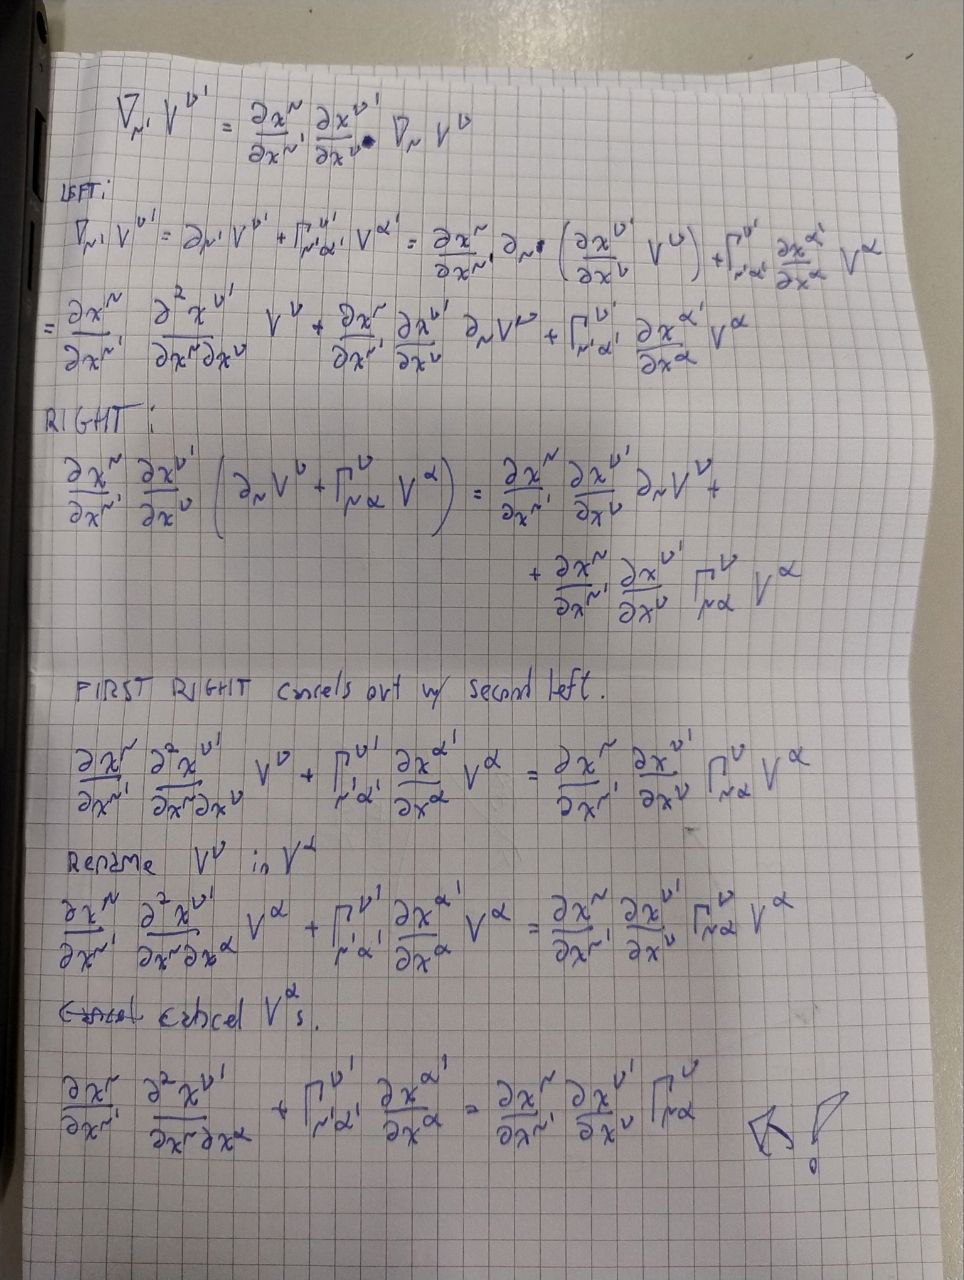
\includegraphics[width=0.8\linewidth]{imm/conntransf.jpg}
\caption{Same derivation but on paper. If you have any doubts compare with this one.}
\label{imm:conntransf}
\end{figure}
We see that $\Gamma $ is not a tensor because of this extra piece after the transformation.\par
We saw that for a \emph{vector} the covariant derivative acts like
\[
\nabla_{\mu }V^{\nu } = \partial_{\mu }V^{\nu } + \Gamma ^{\nu }_{\mu \alpha }V^{\alpha }
\]
Instead for a \emph{dual vector} the derivative is defined as
\[
\nabla _{\mu} \omega _{\nu } \equiv \partial_{\mu }\omega _{\nu } + \tilde{\Gamma }^{\alpha }_{\mu \nu }\omega _{\alpha }
\]
The question that arises from this is obvious: \emph{how $\tilde{\Gamma }$ is related to $\Gamma $?}\par
Let's compute 
\[
\nabla _{\mu }\left( \omega _{\lambda }V^{\lambda } \right) = \partial_{\mu } \left( \omega _{\lambda }V^{\lambda } \right)
\]
This because the covariant derivative of a scalar \emph{is} the derivative of a scalar. So, applying the Leibniz Rule:
\begin{gather*}
\nabla _{\mu }V^{\lambda }\cdot \omega _{\lambda } + V^{\lambda }\nabla _{\mu }\omega _{\lambda } = \partial_{\mu }V^{\lambda }\omega _{\lambda } + V^{\lambda }\partial_{\mu }\omega _{\lambda } \\
\left( \partial_{\mu }V^{\lambda } + \Gamma ^{\lambda }_{\mu  \alpha }V^{\alpha } \right)\omega _{\lambda } + V^{\lambda }\left( \partial_{\mu }\omega _{\lambda } + \tilde{\Gamma }^{\alpha }_{\mu  \lambda } \omega _{\alpha } \right) = \left( \partial_{\mu }V^{\lambda } \right)\omega _{\lambda }+ \left( \partial_{\mu }\omega _{\lambda } \right)V^{\lambda }\\
\to  \Gamma ^{\lambda }_{\mu  \alpha }V^{\alpha }\omega _{\lambda } + \tilde{\Gamma }^{\alpha }_{\mu \lambda } V^{\lambda }\omega _{\alpha } = 0 \\
\text{ renaming some indices to get }\\
\Gamma ^{\lambda }_{\mu \alpha }V^{\alpha }\omega _{\lambda } + \tilde{\Gamma }^{\lambda }_{\mu  \alpha } V^{\alpha }\omega _{\lambda } \\
\implies \Gamma ^{\lambda }_{\mu \alpha } + \tilde{\Gamma }^{\lambda }_{\mu  \alpha } = 0
\end{gather*}

To conclude, the covariant derivative of a dual vector is actually
\begin{equation}
\nabla _{\mu }\omega_{\nu  }= \partial_{\mu }\omega _{\nu } - \Gamma ^{\alpha }_{\mu \nu }\omega _{\alpha }
\end{equation}
 























